\documentclass[conference]{IEEEtran}
\usepackage{graphicx}
\usepackage{booktabs}
\usepackage{amsmath}
\usepackage{url}
\usepackage{cite}

\begin{document}

\title{Empirical Study of Refresh-Token Rotation and Reuse Detection\\
Under Concurrent Requests}

\author{
\IEEEauthorblockN{Albena Veseli, Ardit Hyseni, Erblin Syla}
\IEEEauthorblockA{Group 9 --- Information Security\\
University of Prishtina | Faculty of Electrical and Computer Engineering\\
Email: albena.veseli@student.uni-pr.edu, ardit.hyseni5@student.uni-pr.edu, erblin.syla@student.uni-pr.edu}
}

\maketitle

\begin{abstract}
OAuth 2.0 Security Best Current Practice (RFC 9700) recommends refresh-token
rotation and reuse detection to limit the impact of a stolen refresh token,
but the practical behavior of these mechanisms under \emph{concurrent}
refresh requests is implementation-dependent. We built a small authentication
service implementing four refresh-token strategies --- static (no rotation),
naive rotation (non-atomic read-then-write), atomic rotation
(compare-and-set), and atomic rotation with a reuse grace window --- and a
concurrency test harness that runs four scenarios: client refreshes first,
attacker refreshes first, both refresh concurrently, and the old token is
replayed after a delay. We measured attacker success, access tokens
obtained after compromise, reuse detection, token-family forking, and
legitimate-session survival over 200 trials per configuration (95\% Wilson
confidence intervals reported throughout), and ran the same four scenarios
against two real open-source authorization servers, Keycloak and Ory
Hydra, running locally.
Naive rotation forks the token family in 100\% [98\%, 100\%] of concurrent
races with \emph{zero} reuse alerts, a silent compromise that sequential
testing alone would not reveal. Atomic rotation detects every race but
always revokes the legitimate session along with the attacker's, since the
two cannot be told apart. A reuse grace window reproduces the same silent
takeover as naive rotation whenever the attacker replays inside the window.
Against real servers, we reproduced CVE-2026-1035 on Keycloak 26.2.5: two
simultaneous refreshes of one token both succeeded in 51\% [41\%, 61\%] of
trials, and in almost every such fork both resulting token chains stayed
valid, as with our naive strategy. The race window narrows as more requests compete
(0\% [0\%, 7\%] at 10 concurrent requests). Ory Hydra v26.2.0 also
accepted one token more than once under concurrency (98\% [90\%, 100\%] of
trials at 10 concurrent requests). After such a fork, Hydra keeps at most
the chain that is used first, so an attacker who refreshes again before
the client can take over the session and lock the client out. With Hydra's own
reuse grace period enabled,
a replay inside the window succeeded silently in 100\% [84\%, 100\%] of
trials, confirming the grace-window takeover on a real server.
\end{abstract}

\section{Introduction}

Refresh tokens allow applications to maintain long-lived user sessions
without keeping access tokens valid for long periods. If a refresh token is
stolen, an attacker may use it to obtain new access tokens and continue
accessing resources on behalf of the user. RFC~9700 recommends refresh-token
rotation and reuse detection as a way of detecting the replay of a
compromised refresh token \cite{rfc9700}: a new refresh token is issued
after each successful refresh, the previous token is no longer accepted, and
reuse of an already-invalidated token signals compromise. The OAuth 2.0
threat model discusses the same risk \cite{rfc6819}.

While RFC~9700 establishes rotation and reuse detection as recommended
measures, their behavior under \emph{concurrent} refresh requests is
implementation-dependent. The interaction between checking a token's state,
updating that state, and concurrent requests can determine whether reuse is
detected consistently. This is not merely hypothetical: CVE-2026-1035
\cite{cve} in Keycloak is a time-of-check-to-time-of-use (TOCTOU) flaw in which concurrent
requests could each exchange the same refresh token for a valid access
token before the usage state was updated, bypassing single-use enforcement.
More generally, a legitimate client and an attacker may send requests with
the same refresh token at nearly the same time, and the outcome may depend
on whether the implementation performs a simple read-then-write operation
or an atomic state transition.

To our knowledge, no peer-reviewed empirical study has systematically
measured this behavior across real implementations. Recent
specification-level treatments of refresh-token rotation explicitly leave
this empirical characterization as open work, making no claim about how
often such race conditions occur in deployed systems \cite{nebula}. The
foundational formal analysis of OAuth~2.0 \cite{fett2016} deliberately
excludes token expiration and revocation, and fuzzing frameworks such as
OAuthFuzz \cite{oauthfuzz} aim to discover unknown logic bugs rather than
measure a specific mechanism under concurrency.

The main research question investigated in this paper is:

\begin{quote}
\emph{How do different refresh-token rotation strategies affect reuse
detection, legitimate-session survival, and performance under concurrent
refresh requests?}
\end{quote}

A secondary question is whether a configured grace window (a short interval
during which a just-rotated token is still accepted, intended to tolerate
lost responses) enables a \emph{silent takeover}, in which an attacker
obtains a valid token family with no reuse alert raised.

\section{Related Work}

RFC~9700 \cite{rfc9700} and the earlier OAuth 2.0 threat model
\cite{rfc6819} establish rotation and reuse detection as recommended
countermeasures against refresh-token compromise, but are specification
documents and do not measure implementation behavior. Fett et al.
\cite{fett2016} give a comprehensive formal security analysis of OAuth~2.0,
but explicitly exclude token expiration and revocation from their model.
NEBULA \cite{nebula} gives a language-independent specification for opaque
rotating refresh tokens and explicitly leaves empirical measurement of race
conditions in deployed systems as open work. OAuthFuzz \cite{oauthfuzz} is
a protocol-aware fuzzer for OAuth~2.0 implementations aimed at discovering
unknown logic bugs, rather than measuring the behavior of a specific,
known mechanism under controlled concurrency. This project sits in the gap
between these: a controlled, repeatable measurement of one specific,
already-documented mechanism (rotation and reuse detection) under
concurrency, validated against real server implementations.

\section{Methodology}

\subsection{Rotation strategies}

We implemented a small FastAPI authentication service backed by a
pluggable token store (in-memory or Redis), with four interchangeable
refresh-token strategies:

\begin{itemize}
\item \textbf{Static}: the refresh token is never rotated and can be
reused indefinitely. This is the baseline.
\item \textbf{Naive rotation}: the token's status is read, checked, and
then written back as two separate store operations (a classic
time-of-check-to-time-of-use pattern), with an optional configurable delay
between the two steps.
\item \textbf{Atomic rotation}: the token's status is updated with a
single compare-and-set operation (a Lua script under Redis), so only one
concurrent caller can successfully consume a given token. The loser is
treated as a reuse attempt and the whole token family is revoked.
\item \textbf{Grace-window rotation}: atomic rotation, but a token
presented again within a configurable grace window after being consumed is
treated as a benign retry rather than a reuse attempt, and is issued a
fresh token silently, with no alert and no revocation.
\end{itemize}

\subsection{Concurrency harness}

A Python \texttt{asyncio}-based harness simulates a legitimate client and
an attacker who holds a copy of the same stolen refresh token, and drives
four scenarios:

\begin{itemize}
\item \textbf{Sequential replay}: the legitimate client refreshes, then
the attacker presents the now-superseded token.
\item \textbf{Attacker-first replay}: the attacker refreshes first, and the
legitimate client is the one presenting the superseded token.
\item \textbf{Concurrent race}: both parties present the same token at the
same instant, synchronized with an \texttt{asyncio.Event} gate so neither
is systematically scheduled first.
\item \textbf{Delayed replay}: the legitimate client rotates, and the
attacker replays the stolen token after a configurable delay --- used to
probe the boundary of a grace window.
\end{itemize}

For each trial we record whether the attacker obtained a valid access
token, whether a reuse alert was raised, how many live tokens remain in
the token family (more than one indicates \emph{forking}), whether the
token family was revoked, and whether the legitimate client's session
still works afterward. To count the access tokens obtained after
compromise, the attacker then keeps refreshing with whatever token it
holds, up to three more times; a static or forked token chain yields four
tokens, a revoked one yields at most one. Every rate reported in this paper is accompanied by
its 95\% Wilson score confidence interval \cite{wilson1927}, computed from
the number of trials and successes rather than the normal approximation,
since several of our rates sit at or near the 0\%/100\% boundary where the
normal approximation is unreliable.

\subsection{Pilot experiment}

Before the main evaluation we ran a pilot (20 trials per configuration;
static, naive and atomic rotation; sequential replay and concurrent race)
to check that the harness reliably generates concurrent requests and
records token states correctly. The pilot reproduced the expected
signatures: naive rotation forked the family in 20/20 races, atomic
rotation never forked and flagged every race, and the static baseline was
never flagged. Each main experiment was then run on both the in-memory
store and the Redis store; unless stated otherwise, the figures report the
in-memory run, and the Redis run is used as a cross-check.

\subsection{Experimental environment}

All experiments ran on one laptop: Intel Core i7-9850H (6 cores, 12
threads, 2.6\,GHz), 32\,GB RAM, Windows~11 Pro (build 26300), Docker
Engine~28.3.2 (Docker Desktop, WSL\,2 backend, 12 vCPUs and 15.5\,GB
assigned). The service and harness used Python~3.14.3 with FastAPI~0.141.1,
Uvicorn~0.54.0, HTTPX~0.28.1 and redis-py~8.1.0; the token store was
Redis~7 (\texttt{redis:7-alpine}). The service, harness and comparison
servers are all defined in the project's \texttt{docker-compose.yml}; the
containerized service and harness use Python~3.12. All traffic stayed on
the local machine: the harness talked to the servers over
\texttt{localhost} and Docker's default bridge network, with no added
network delay or packet loss.

\subsection{Real-server comparison}

In addition to the controlled implementation, we ran two open-source
OAuth~2.0/OIDC authorization servers locally in Docker: \textbf{Keycloak
26.2.5} (the version associated with CVE-2026-1035, configured with strict
rotation: \texttt{revokeRefreshToken=true}, \texttt{refreshTokenMaxReuse=0})
and \textbf{Ory Hydra v26.2.0} (SQLite-backed, strict rotation by default,
i.e.\ \texttt{rotation\_grace\_period=0s}). For Keycloak we used the
resource-owner password grant to obtain and refresh tokens directly. Hydra
has no password grant, so we drove its authorization-code flow
programmatically against its login/consent \emph{admin} API --- the same
mechanism a real consent application uses, invoked directly rather than
through a browser --- to obtain and refresh tokens for a single test
subject on our own local instance.

Against both servers we ran the same four two-party scenarios as in the
controlled harness (60 trials each; replay delay 1\,s). A real server
does not tell the caller that it detected reuse, so we observe detection
by its effect: after the stale token is presented, we check whether the
successor that \emph{did} rotate still works. If it no longer works, the
server revoked the session, which is the reuse response RFC~9700
recommends. We count attacker tokens with the same three follow-up
refreshes as above. Separately, to see how the race depends on load, we
sent $k$ simultaneous refreshes of one token for
$k \in \{2, 5, 10, 20, 50\}$ (Keycloak) and $k = 10$ (Hydra), and
counted trials where more than one succeeded. Finally, we repeated the
delayed-replay scenario against Hydra with its
\texttt{rotation\_grace\_period} set to 5\,s, at delays of 1, 3 and 6\,s
(20 trials each).

\section{Results}\label{sec:results}

\subsection{Controlled implementation}

Table~\ref{tab:main-results} summarizes the concurrent-race scenario for
each strategy over 200 trials; Fig.~\ref{fig:security} shows the same data
alongside sequential-replay detection, which was 100\% for both rotation
strategies in every configuration tested.

\begin{table}[htbp]
\centering
\caption{Security outcomes under a concurrent refresh race (N=200 trials; brackets show the 95\% Wilson confidence interval).}
\label{tab:main-results}
\begin{tabular}{lccc}
\toprule
Strategy & Attacker success & Reuse detected & Family forked \\
\midrule
static & 100\% [98\%, 100\%] & 0\% [0\%, 2\%] & 0\% [0\%, 2\%] \\
naive rotation & 100\% [98\%, 100\%] & 0\% [0\%, 2\%] & 100\% [98\%, 100\%] \\
atomic rotation & 52\% [45\%, 58\%] & 100\% [98\%, 100\%] & 0\% [0\%, 2\%] \\
\bottomrule
\end{tabular}
\end{table}

\begin{figure}[htbp]
\centering
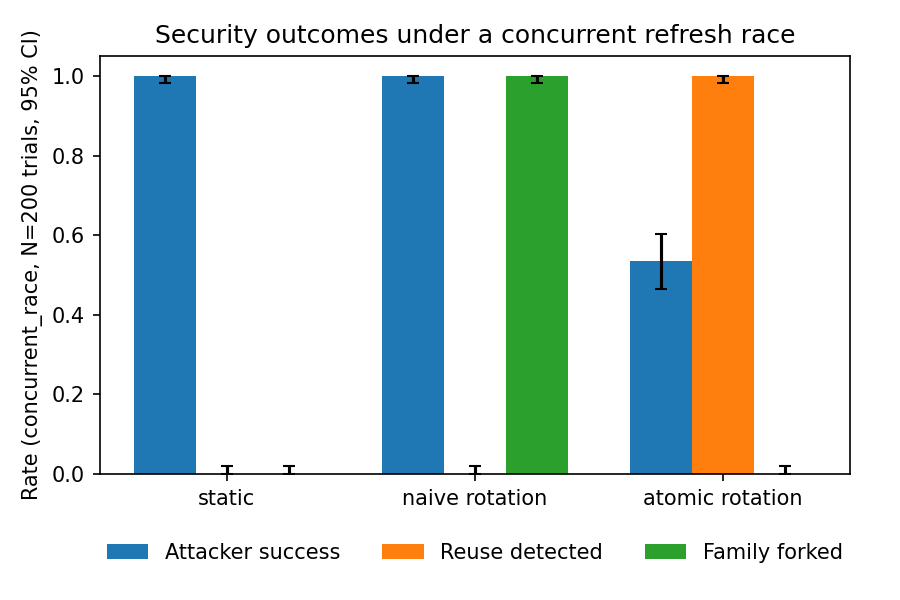
\includegraphics[width=\columnwidth]{figures/security_concurrent_race.png}
\caption{Security outcomes under a concurrent refresh race, by strategy
(N=200 trials each).}
\label{fig:security}
\end{figure}

Static tokens are trivially and permanently exploitable: the attacker
succeeds every time and nothing is ever flagged. Naive rotation correctly
detects a \emph{sequential} replay (100\% [98\%, 100\%] detection, median
latency $\approx$27\,\textmu s) but under a true concurrent race it forks
the token family in 100\% [98\%, 100\%] of trials with \emph{zero} reuse
alerts --- both the attacker and the legitimate client receive a valid,
independent successor token, and the compromise is completely silent.
Atomic rotation detects every race (100\% [98\%, 100\%]) and never forks;
the attacker wins the race in 54\% [47\%, 60\%] of trials (consistent
with the 50\% expected from randomized start order --- the 95\% CI
comfortably includes 50\%), but the loser --- whichever party it is --- is
immediately detected and the whole token family, including the legitimate
client's side, is revoked. Widening naive rotation's internal check/use gap
from 0 to 10\,ms had no additional effect on the race outcome: it was
already forking in 100\% of trials at zero added delay. In the in-memory
store this is because the strategy yields to the event loop once between
check and write (\texttt{asyncio.sleep(0)}); with the Redis store, no
artificial yield is needed, since the network round trip between the read
and the write opens the window naturally, and the result is the same
(100\% fork). The forked chains are durable: in every naive race the
attacker went on to obtain all four access tokens (one in the race plus
three follow-ups), as with static tokens. Under atomic rotation the
attacker obtained 0.54 tokens on average, never more than the one from
the race itself.

The two remaining sequential scenarios behave as expected for every
strategy. When the \emph{attacker} refreshes first, both rotation
strategies flag the client's subsequent use of the stale token in 100\%
[98\%, 100\%] of trials, but the attacker has by then already obtained a
token in every trial, and the resulting family revocation locks out the
legitimate client. Detection therefore always fires, but only after the
attacker has received one access token. A replay of the old token 100\,ms after a
successful rotation is detected in 100\% of trials by both rotation
strategies, while static tokens accept it every time.

\subsection{Grace window (secondary research question)}

Fig.~\ref{fig:grace} shows the silent-compromise rate as a function of how
long after rotation the attacker replays the stolen token, for atomic
rotation (no grace window) versus grace-window rotation (50\,ms window).

\begin{figure}[htbp]
\centering
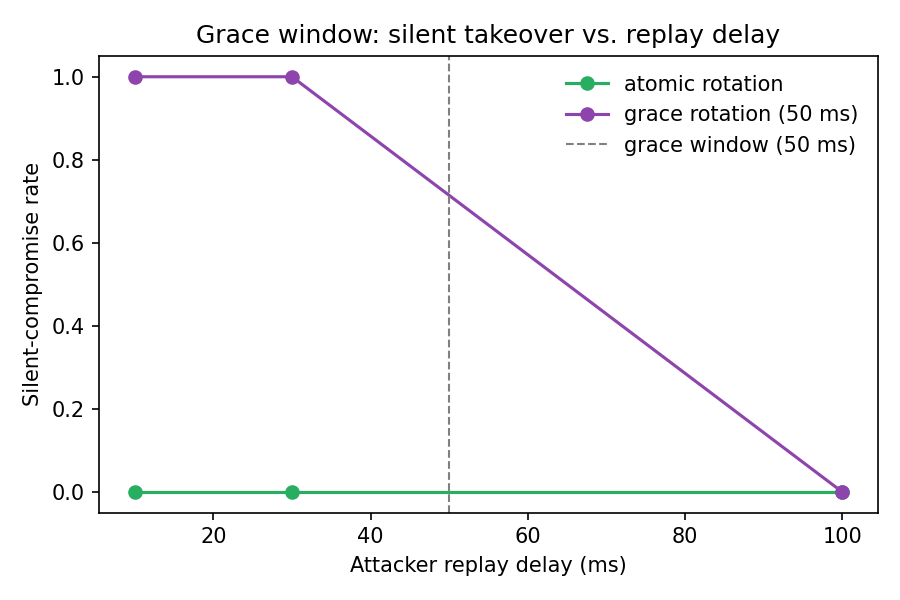
\includegraphics[width=\columnwidth]{figures/grace_window_takeover.png}
\caption{Silent-compromise rate vs.\ attacker replay delay, with and
without a 50\,ms reuse grace window (N=100 trials per point).}
\label{fig:grace}
\end{figure}

Atomic rotation detects a replay at every delay tested. Grace-window
rotation silently admits the attacker in 100\% of trials when the replay
falls inside the 50\,ms window (10\,ms and 30\,ms delays) and correctly
detects it in 100\% of trials once the delay exceeds the window
(100\,ms). This directly confirms the secondary research question: a
configured grace window enables a silent token-family takeover, with no
reuse alert raised, for any attacker fast enough to replay within it.
The Redis cross-check agrees at 10\,ms and 100\,ms. At 30\,ms the rate
drops to 79\% [70\%, 86\%], because each Redis round trip uses up part of
the 50\,ms window and the effective window is therefore shorter. With the
Redis store, the atomic race was won by the attacker in 53\% [46\%, 59\%] of
trials, again with 100\% detection and no forking.

\subsection{Performance}

Fig.~\ref{fig:latency} shows single-client, real-HTTP refresh latency
(median of 5 repeated runs, error bars show min/max) for each strategy
against the deployed FastAPI service with a Redis backend.

\begin{figure}[htbp]
\centering
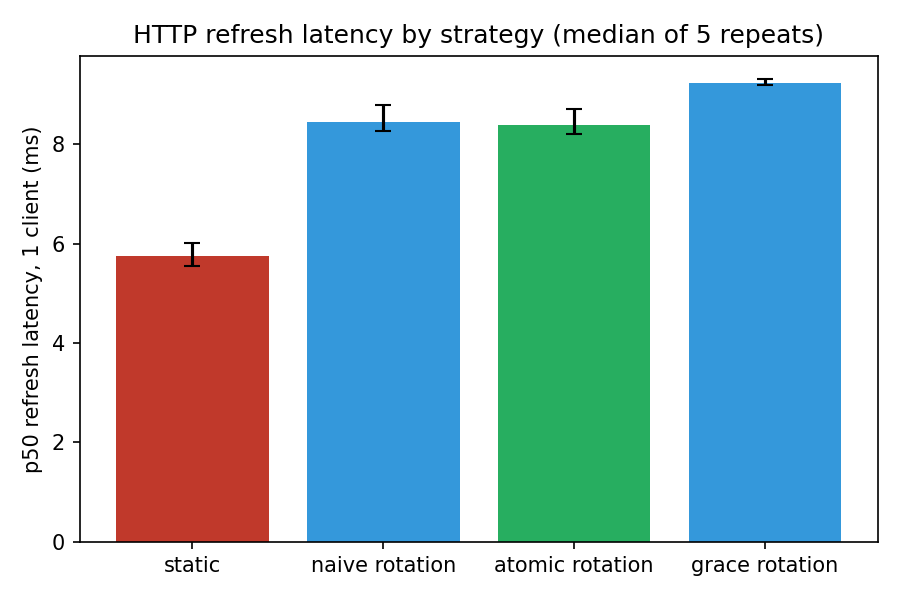
\includegraphics[width=\columnwidth]{figures/benchmark_latency.png}
\caption{Single-client p50 refresh latency by strategy over real HTTP.}
\label{fig:latency}
\end{figure}

Rotation costs roughly 2.7\,ms over the static baseline (5.75\,ms vs.\
8.4\,ms), reflecting the extra Redis write needed to persist a new token
record. Critically, atomic rotation (8.38\,ms) shows no measurable cost
over naive rotation (8.44\,ms): making the state transition atomic is
effectively free, so the security gain comes at no latency penalty.
Grace-window rotation costs a further $\sim$0.8\,ms (9.23\,ms) for the
additional timestamp write needed to track the grace period. Under
10 concurrent clients, throughput converged to $\approx$175\,requests/s
for all four strategies, indicating the deployment (one \texttt{uvicorn}
worker on a single machine) rather than any strategy was the bottleneck
at that load; we therefore do not draw strategy comparisons from the
multi-client results.

Fig.~\ref{fig:resources} reports the server process's mean CPU usage and
resident memory (RSS) under the single-client load, sampled every 50\,ms
with \texttt{psutil} and averaged over the same 5 repeated runs.

\begin{figure}[htbp]
\centering
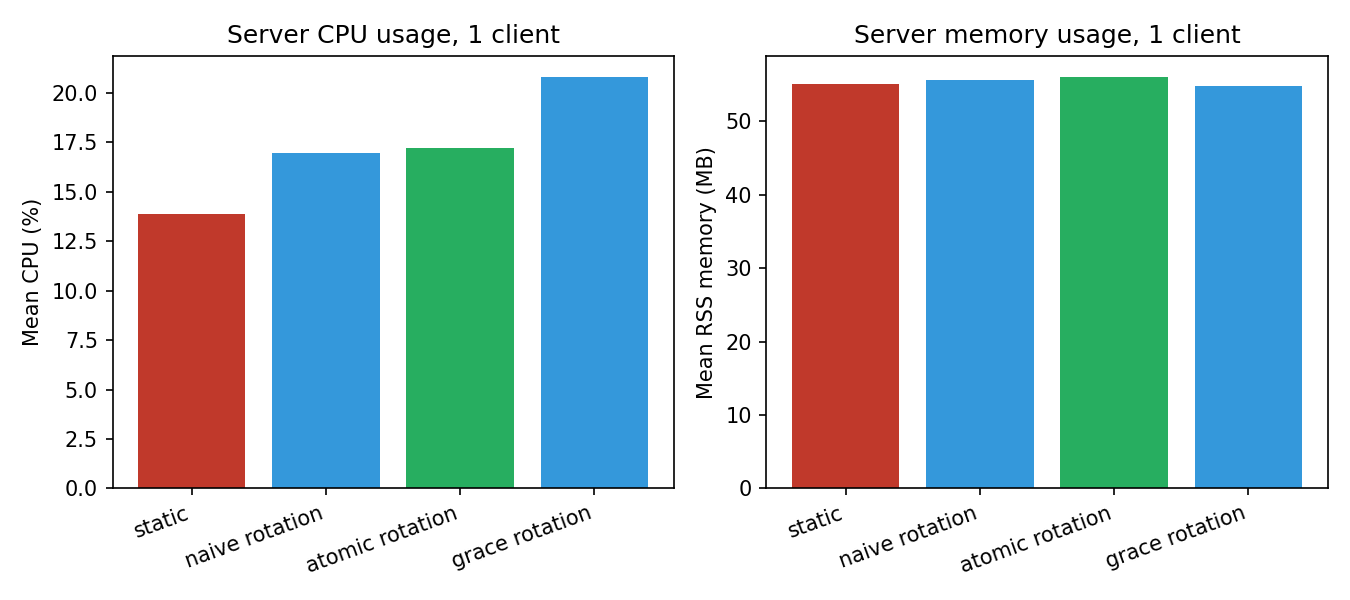
\includegraphics[width=\columnwidth]{figures/benchmark_resources.png}
\caption{Server-process CPU and memory usage by strategy, single client,
median of 5 repeated runs.}
\label{fig:resources}
\end{figure}

Resident memory is flat across all four strategies (54.8--56.1\,MB),
confirming that the baseline Python/uvicorn/FastAPI process footprint
dominates and that none of the strategies hold meaningfully more state in
memory than any other --- unsurprising, since every strategy's per-token
state lives in Redis, not in the server process. Mean CPU usage ranges
from 13.9\% (static) to 20.8\% (grace rotation) and roughly tracks each
strategy's per-request latency rather than suggesting a fundamentally
different algorithmic cost: a strategy that takes longer per request
keeps the single-threaded event loop busy longer per request, which
\texttt{psutil} reports as higher CPU occupancy, even though the
underlying work (one or two small Redis operations) is comparable across
strategies. We therefore do not read these figures as evidence that any
rotation strategy is computationally expensive in an absolute sense; the
CPU/memory comparison instead supports the same conclusion as the latency
results, that the cost of atomicity and the grace window is small and
dominated by I/O to the token store rather than CPU-bound computation.

\subsection{Real-server comparison}

Table~\ref{tab:server-scenarios} reports the four scenarios against both
servers, and Table~\ref{tab:real-server} the race at different levels of
concurrency.

\begin{table*}[htbp]
\centering
\caption{The four scenarios against real servers (two parties, 60 trials each; 95\% Wilson CI). \emph{Revoked}: the successor that did rotate stopped working after the stale token was presented, i.e.\ reuse was detected. \emph{Attacker tokens}: mean access tokens obtained, including up to three follow-up refreshes. The client and attacker are probed afterwards in random order.}
\label{tab:server-scenarios}
\begin{tabular}{llcccccc}
\toprule
Server & Scenario & Attacker success & Forked & Revoked & Client survives & Attacker survives & Attacker tokens \\
\midrule
Keycloak & Client first & 0\% [0\%, 6\%] & 0\% [0\%, 6\%] & 100\% [94\%, 100\%] & 0\% [0\%, 6\%] & 0\% [0\%, 6\%] & 0.00 \\
Keycloak & Attacker first & 100\% [94\%, 100\%] & 0\% [0\%, 6\%] & 100\% [94\%, 100\%] & 0\% [0\%, 6\%] & 0\% [0\%, 6\%] & 1.00 \\
Keycloak & Concurrent & 70\% [57\%, 80\%] & 48\% [36\%, 61\%] & 52\% [39\%, 64\%] & 43\% [32\%, 56\%] & 45\% [33\%, 58\%] & 2.05 \\
Keycloak & Delayed (1\,s) & 0\% [0\%, 6\%] & 0\% [0\%, 6\%] & 100\% [94\%, 100\%] & 0\% [0\%, 6\%] & 0\% [0\%, 6\%] & 0.00 \\
\midrule
Hydra & Client first & 0\% [0\%, 6\%] & 0\% [0\%, 6\%] & 100\% [94\%, 100\%] & 0\% [0\%, 6\%] & 0\% [0\%, 6\%] & 0.00 \\
Hydra & Attacker first & 100\% [94\%, 100\%] & 0\% [0\%, 6\%] & 100\% [94\%, 100\%] & 0\% [0\%, 6\%] & 0\% [0\%, 6\%] & 1.00 \\
Hydra & Concurrent & 100\% [94\%, 100\%] & 100\% [94\%, 100\%] & 0\% [0\%, 6\%] & 22\% [13\%, 34\%] & 22\% [13\%, 34\%] & 1.65 \\
Hydra & Delayed (1\,s) & 0\% [0\%, 6\%] & 0\% [0\%, 6\%] & 100\% [94\%, 100\%] & 0\% [0\%, 6\%] & 0\% [0\%, 6\%] & 0.00 \\
\bottomrule
\end{tabular}
\end{table*}


\begin{table}[htbp]
\centering
\caption{Concurrent-race reproduction against real authorization servers (brackets show the 95\% Wilson confidence interval).}
\label{tab:real-server}
\begin{tabular}{lcc}
\toprule
Server & Trials & Family fork rate \\
\midrule
Keycloak 26.2.5 & 50 & 0\% [0\%, 7\%] \\
Ory Hydra v26.2.0 & 50 & 96\% [87\%, 99\%] \\
\bottomrule
\end{tabular}
\end{table}

\emph{Sequential scenarios.} Both servers behave like our atomic
strategy. A stale token presented after a successful rotation (client
first, or 1\,s later) is rejected with HTTP~400 \texttt{invalid\_grant}
in 100\% [94\%, 100\%] of trials, and the reuse also kills the client's
freshly rotated token: the session is revoked. When the attacker
refreshes first, the attacker always gets one access token, the client's
later attempt is rejected, and the attacker's new token is then revoked
too, so the attacker obtains exactly one token and the client loses its
session.

\emph{Concurrent race, Keycloak.} Keycloak 26.2.5, configured as
described for CVE-2026-1035 (strict rotation,
\texttt{refreshTokenMaxReuse=0}), let two simultaneous refreshes of one
token both succeed in 51\% [41\%, 61\%] of 100 trials. This reproduces
the CVE. In the two-party scenario, 48\% [36\%, 61\%] of races forked,
and in almost every forked trial both chains stayed valid: afterwards the
attacker could still refresh in 27 of 29 forks and the client in 26 of
29, whichever of them refreshed first. On average, the attacker obtained 2.05
access tokens per race. This is the same silent, durable fork as our
naive strategy. In the other trials,
exactly one request won and the server revoked the session, like our
atomic strategy. The race window narrows as more requests compete: the
fork rate falls to 7\% [2\%, 21\%] at 5 simultaneous requests and 0\% at
10 or more. A likely explanation is that, under heavier contention, the
requests are serialized by database locking before they reach the
vulnerable check. Under this pattern, the attack is most effective in
exactly the realistic case of one attacker racing one client.

\emph{Concurrent race, Hydra.} Ory Hydra accepted one token more than
once in 98\% [90\%, 100\%] of trials at 10 concurrent requests (typically
2--3 of the 10 succeeded), and in 100\% [94\%, 100\%] of two-party races.
Unlike Keycloak, both chains never survive together. Because the order in
which the two parties refresh again is randomized, we can see that the
chain used \emph{first} after the fork survived in 26 of 60 trials (43\%),
and the other chain was revoked in every trial; in the remaining trials
both were revoked. When the attacker refreshed first, the attacker kept a
working chain in 13 of 24 trials and the client was locked out in all 24.
Hydra thus appears to detect the double use only when the second chain is
used, and by then it may revoke the legitimate client instead of the
attacker. Our first version of this measurement always probed the client
first and therefore wrongly suggested that the attacker's chain always
dies; randomizing the order corrected this.

\emph{Grace window, Hydra.} With \texttt{rotation\_grace\_period=5s},
a replay 1\,s or 3\,s after rotation succeeded silently in 100\% [84\%,
100\%] of 20 trials each, and the client's session survived, exactly
reproducing the silent takeover of our grace-window strategy. A replay
at 6\,s was rejected in 100\% of trials and revoked the client's
already-rotated token as well (client survival 0\% [0\%, 16\%]), the
same trade-off as our atomic strategy.

\section{Discussion}

The central finding is that \emph{sequential} testing of rotation and
reuse detection, which is what most informal testing and manual QA would
naturally perform, is insufficient to characterize security under
concurrency: naive rotation passes every sequential test perfectly (100\%
detection) while failing every concurrent one (100\% silent fork). A
system that appears secure under the OAuth BCP's stated threat model can
still be fully compromised by an attacker capable of racing a single
request against the legitimate client, with no observable trace in server
logs or alerts.

The atomic strategy's trade-off is equally important to state plainly:
making reuse detection reliable under concurrency does not mean the
attacker never wins the race ($\approx$54\% of the time, they do, since the
server cannot distinguish the two parties by anything other than arrival
order), but it does mean the loser is always detected and the family is
always revoked --- including the legitimate client's side. This matches
behavior we also observed on Ory Hydra: detected reuse outside its grace
window revoked the legitimate client too. This is consistent with the
recommended response in RFC~9700, but it means atomic rotation alone
converts an attacker's successful race into a denial-of-service against
the legitimate user, not into a silent, cost-free defense.

Reproducing CVE-2026-1035 validates the harness, as the proposal
intended: the same two-party race that exposes our naive strategy also
exposes a known real-world TOCTOU flaw, over ordinary HTTP on a single
node. The result also shows why the outcome must be reported as a rate
with a confidence interval rather than as a single pass or fail. The race
succeeds in roughly half of two-request trials, and a test that sends
many requests at once (10 or more) would miss it entirely and wrongly
conclude that the server is safe. Red Hat rates the CVE's attack
complexity as ``high''; our data suggest that, for an attacker who already
holds the token, the timing is easier to hit than that rating implies.
The two real servers also fail in different ways. Keycloak's fork is
durable: like naive rotation, both the attacker and the client keep a
working chain and nothing is flagged. Hydra's fork resolves to whichever
party refreshes next. This is a race the attacker can win simply by
refreshing immediately, which turns the double use into a session
takeover in which the legitimate client, not the attacker, is locked out.
Both break single-use enforcement, and in both the attacker can end up
with lasting access.

\subsection{Responsible disclosure}

The Ory Hydra result (Sec.~\ref{sec:results}) shows that a single refresh
token can be exchanged more than once under concurrency, even with strict
rotation, and that an attacker who refreshes first after the race can keep
the session while the legitimate client is revoked. In line with the project proposal, we treat this as a potential
defect. We will report it privately to the Ory maintainers through their
security policy before sharing the result outside the course, and will not
publish exploit details until they have had time to respond. At the time
of writing, the report has not yet been submitted. The Keycloak
behaviour concerns an already-published CVE and needs no new report.

\section{Limitations}

Results depend on the specific versions, configurations, and storage
backends of the tested systems (Keycloak~26.2.5, Ory Hydra~v26.2.0,
Redis~7, SQLite for Hydra) and should not be treated as universal
properties of all OAuth~2.0 authorization servers or of later versions.
Both real-server deployments were single-node development instances; a
clustered or high-load production deployment could plausibly open race
windows that do not appear here, particularly for Keycloak. All testing
targeted only our own local, containerized systems with synthetic
clients; no real users or third-party services were involved. The project
assumes a refresh token has already been compromised and does not
investigate how it was obtained (XSS, malware, and device compromise are
out of scope). Concurrency results can be affected by the host operating
system, hardware, and scheduling; all experiments here were run on a
single Windows machine with Docker Desktop, which we note for
reproducibility rather than as a controlled variable. The 200/100-trial
security experiments and the real-server validation were each run once,
not repeated across separate sessions; the reported confidence intervals
quantify sampling variability within a single run of $N$ trials but not
variability across different machine states, times of day, or reboots.
CPU and memory sampling (Fig.~\ref{fig:resources}) measures only the
server process's own usage at a 50\,ms polling interval on a single
machine; it does not account for Redis's or Docker's own resource
consumption, and the sampling interval is too coarse to attribute usage
to individual requests.

\section{Conclusion}

We built a controlled refresh-token rotation testbed and concurrency
harness and used it to show that non-atomic (naive) rotation, despite
passing all sequential reuse-detection tests, silently forks the token
family in 100\% of concurrent races with no alert raised, while atomic
(compare-and-set) rotation detects every race at a measured latency cost
of effectively zero over the naive implementation. A reuse grace window,
intended to tolerate lost responses, reproduces the same silent-takeover
failure mode whenever an attacker can replay within the window, both in
our own implementation and against Ory Hydra's equivalent setting.
Running the same scenarios against two real authorization servers
reproduced CVE-2026-1035 on Keycloak~26.2.5 (51\% of two-request races
forked, with both chains staying valid), but only at low concurrency, and
showed a double use on Ory Hydra in which whichever party refreshes next
keeps the session, so an attacker can take it over. On both servers, a detected
sequential reuse revoked the legitimate session as well, the same
security/availability trade-off as our own atomic strategy. These
results support preferring atomic, compare-and-set token-state transitions
over read-then-write rotation, and avoiding reuse grace windows unless
their silent-takeover exposure is explicitly accepted.

\begin{thebibliography}{5}

\bibitem{rfc9700}
T. Lodderstedt, J. Bradley, A. Labunets, and D. Fett, ``Best Current
Practice for OAuth 2.0 Security,'' RFC 9700, IETF, Jan. 2025. [Online].
Available: \url{https://www.rfc-editor.org/rfc/rfc9700.html}

\bibitem{rfc6819}
T. Lodderstedt, M. McGloin, and P. Hunt, ``OAuth 2.0 Threat Model and
Security Considerations,'' RFC 6819, IETF, Jan. 2013. [Online]. Available:
\url{https://www.rfc-editor.org/rfc/rfc6819.html}

\bibitem{nebula}
M. Teodori, ``NEBULA: A Language-Independent Specification for Opaque
Rotating Refresh Tokens,'' arXiv:2608.04115, Aug. 2026. [Online].
Available: \url{https://arxiv.org/abs/2608.04115}

\bibitem{fett2016}
D. Fett, R. K\"usters, and G. Schmitz, ``A Comprehensive Formal Security
Analysis of OAuth 2.0,'' in \emph{Proc. ACM SIGSAC Conf. Computer and
Communications Security (CCS)}, 2016, pp. 1204--1215.

\bibitem{oauthfuzz}
G. Zhang et al., ``OAuthFuzz: Protocol-Aware Adaptive Fuzzing for OAuth
2.0 Implementations,'' preprint, SSRN 7094132, 2026.

\bibitem{cve}
Red Hat, ``CVE-2026-1035,'' Red Hat CVE Database, Jan. 2026. [Online].
Available: \url{https://access.redhat.com/security/cve/CVE-2026-1035}

\bibitem{wilson1927}
E. B. Wilson, ``Probable Inference, the Law of Succession, and Statistical
Inference,'' \emph{Journal of the American Statistical Association},
vol. 22, no. 158, pp. 209--212, 1927.

\end{thebibliography}

\end{document}